% Le modèle de Thomas

\section{Le Modèle de Thomas}
\seclabel{thomas}

Nous présentons dans cette section le \emph{modèle de Thomas} (\secref{thomas-def}),
historiquement très utilisé dans la représentation des réseaux de régulation biologique.
Il s'agit d'un modèle asynchrone basé sur un \emph{graphe des interactions} et
une carte de \emph{paramètres} discrets.
Les \emph{réseaux discrets asynchrones} sont aussi définis (\secref{rda-def})
du fait de leurs similitudes avec le modèle de Thomas.
Nous proposons enfin un rapide tour d'horizon des différentes méthodes utilisées
pour analyser la dynamique de ces modèles (\secref{thomas-analyse}).

\subsection{Définition du modèle de Thomas}
\seclabel{thomas-def}

Le modèle dit \emph{de Thomas} a été théorisé et proposé pour la première
fois par \citefullname{Thomas73}{René} dans le but d'abstraire les systèmes
d'équations différentielles permettant la représentation de réseaux de régulation biologique.
Son intuition était de proposer une simplification discrète cohérente de ces systèmes
afin de permettre des analyses plus efficaces.
Nous proposons ici une définition inspirée de divers travaux plus récents,
comportant notamment des paramètres discrets \cite{Snoussi89}
%des composants multivalués \cite{Richard06,BernotSemBRN}
et des arcs non-signés \cite{FPIMR12-CMSB}.

\myskip

% Paramètres de Snoussi : \cite{Snoussi89}
% SMBionet : \cite{Richard06}
% Hypothèses d'activité et monotonicité : \cite{BernotSemBRN}

Un modèle de Thomas représente un ensemble fini de composant se régulant entre eux.
Ces composants sont décrits par un niveau d'expression discret qui
caractérise leur état (taux d'activité pour un gène, concentration pour une protéine, etc.).
Afin de représenter la structure d'un tel système,
on utilise généralement un \emph{graphe des interactions} (\defref{thomas-gi})
dont les nœuds représentent un ensemble de composants
et les arcs (orientés) leurs influences mutuelles.
Les nœuds sont étiquetés par un nom (celui du composant : $a$, $b$, $c$, etc.)
et un plafond (son niveau d'expression maximum : $l_a$, $l_b$, $l_c$, etc.).
Les arcs sont de la forme : $\arc{a}{s}{t}{b}$,
c'est-à-dire étiquetés par un signe $s$ qui représente le type de régulation
($+$ pour une activation, $-$ pour une inhibition
et $\uns$ pour une régulation plus complexe)
et un entier $t$ qui représente le seuil de déclenchement de la réaction
(c'est-à-dire le niveau d'expression du composant régulateur à partir duquel celui-ci
a effectivement une influence sur le composant régulé).
Bien que plusieurs variantes aient été proposées,
nous nous intéressons ici à une définition où
chaque arc est unique, c'est-à-dire qu'il ne peut pas exister deux arcs
$\arc{a}{s}{t}{b}$ et $\arc{a}{s'}{t'}{b}$ étiquetés différemment dans le graphe.
L'utilité des arcs non-signés ($\uns$) est discutée à la fin de cette section.

\begin{definition}[Graphe des interactions]
\deflabel{thomas-gi}
  Un \emph{graphe des interactions} est un couple $\GI = (\components; E)$ où
  $\components$ est l'ensemble fini des \emph{composants},
  étiquetés par un nom et un \emph{plafond},
  et $E$ est l'ensemble fini des \emph{régulations} entre deux nœuds,
  étiquetées par un \emph{signe} et un \emph{seuil} :
    \[E \DEF \{ \arc{a}{s}{t}{b}, \ldots \mid
      a, b \in \components \wedge s \in \{ +, -, \uns \} \wedge t \in \segm{1}{l_a}\}\]
  tel que chaque régulation de $a$ vers $b$ soit unique :
    \[\forall \arc{a}{s}{t}{b} \in E,
      \forall \arc{a}{s'}{t'}{b} \in E, s = s' \wedge t = t' \enspace.\]
\end{definition}
%
Étant donnée cette définition, on note
$E_s \DEF \{ \arc{a}{s}{t}{b} \in E \}$ pour $s \in \{ +, -, \uns \}$.
De plus, pour tout composant $b \in \components$, on note $\RRBreg{b}$ l'ensemble de ses
\emph{régulateurs} :
    \[\RRBreg{b} \DEF \{ a \in \components \mid \exists \arc{a}{s}{t}{b} \in E \}\]
\label{regulateurs}

\begin{example}
  La \figref{thomas}(gauche) représente un graphe des interactions $(\components; E)$ où
  $\components = \{a, b, c\}$, avec $l_a = 2$ et $l_b = l_c = 1$, et :
  \begin{align*}
    E_+ &= \{\arc{b}{+}{1}{a}, \arc{c}{+}{1}{a}\} &
    E_\uns &= \emptyset \\
    E_- &= \{\arc{a}{-}{2}{b}\}
  \end{align*}
  Ainsi :
  \begin{align*}
    \RRBreg{a} &= \{ b, c \} &
    \RRBreg{b} &= \{ a \} \\
    \RRBreg{c} &= \emptyset
  \end{align*}
  Pour des raisons d'illustration, le composant $a$ ne comporte aucun arc sortant avec le seuil
  $1$, mais possède un arc sortant étiqueté avec le seuil $2$.
  Ce type de configuration ne se rencontre habituellement pas dans les modèles de Thomas
  pour des raisons discutées \vpageref{plafond}.
  
  \begin{figure}[ht]
    \begin{minipage}{0.49\textwidth}
    \centering
    \scalebox{1.2}{
    \begin{tikzpicture}[grn]
      \path[use as bounding box] (-0.3,-0.75) rectangle (4,.75);
      \node[inner sep=0] (a) at (2,0) {a};
      \node[inner sep=0] (b) at (0,0) {b};
      \node[inner sep=0] (c) at (3.8,0) {c};
      
      \node[elabel, below=-.8em of a] {$0..2$};
      \node[elabel, below=-.8em of b] {$0..1$};
      \node[elabel, below=-.8em of c] {$0..1$};
      
      \path[->]
        (b) edge[bend right] node[elabel, below=-5pt] {$+1$} (a)
        (c) edge node[elabel, above=-5pt] {$+1$} (a)
        (a) edge[bend right] node[elabel, above=-5pt] {$-2$} (b);
    \end{tikzpicture}
    }
    \end{minipage}
    \begin{minipage}{0.49\textwidth}
    \centering
    \begin{align*}
      K_{a,\emptyset} &= \segm{0}{0} & K_{b,\emptyset} &= \segm{0}{1} \\
      K_{a,\{b\}} &= \segm{1}{1} & K_{b,\{a\}} &= \segm{0}{0} \\
      K_{a,\{c\}} &= \segm{1}{1} &&\\
      K_{a,\{b,c\}} &= \segm{2}{2} & K_{c,\emptyset} &= \segm{0}{1}
    \end{align*}
    \end{minipage}
    \caption{\figlabel{thomas}%
      (gauche)
        Un exemple de graphe des interactions.
        Les composants sont représentés par les nœuds, comportant un nom et un
        ensemble de niveaux d'expression,
        tandis que les régulations sont représentées par des arcs
        étiquetés par un signe et un seuil.
        Par exemple, l'arc de $b$ vers $a$ étiqueté $+1$ représente la régulation $\arc{b}{+}{1}{a}$.
        En d'autres termes, $b$ se comporte comme un activateur de $a$ si son niveau d'expression
        est égal à $1$, et se comporte comme un inhibiteur sinon (c'est-à-dire si son niveau
        d'expression est égal à $0$).
      (droite)
        Un exemple de paramétrisation du graphe des interactions de gauche.
    }
  \end{figure}
\end{example}

Pour tout composant $a$ régulant $b$, c'est-à-dire si $\arc{a}{s}{t}{b} \in E$,
on note $\levels{a}{b}$ (\resp $\ulevels{a}{b}$) l'ensemble des niveaux d'expression
de $a$ qui sont au-dessus (\resp en-dessous) du seuil $t$ (\defref{levels}).
Au niveau de la dynamique,
pour tout niveau d'expression de $a$ appartenant à $\levels{a}{b}$, $a$ est censé avoir
une influence correspondant au signe $s$ sur $b$,
c'est-à-dire être activateur si $s = +$, inhibiteur si $s = -$,
ou avoir une influence indéterminée ou multiple si $s = \uns$ ;
en revanche, pour tout niveau d'expression de $a$ appartenant à $\ulevels{a}{b}$,
l'influence opposée devrait être observée.
Cette hypothèse permet de modéliser la dégradation de $b$ en l'absence de l'activation de $a$
si $s = +$, ou l'activation de $b$ en l'absence de l'inhibition de $a$ si $s = -$.

\begin{definition}[Niveaux effectifs ($\levelssymbol$)]
\deflabel{levels}
  Soit $\GI = (\components; E)$ un graphe des interactions.
  Si $\arc{a}{s}{t}{b} \in E$, on définit :
    \[\levels{a}{b} \DEF \segm{t}{l_a} \quad \text{et} \quad
      \ulevels{a}{b} \DEF \segm{0}{t-1}\]
\end{definition}

\begin{example}
  Sur le graphe des interactions de la \figref{thomas}(gauche)
  on a notamment :
  \begin{align*}
    \levels{a}{b} &= \segm{2}{2} & \ulevels{a}{b} &= \segm{0}{1}
  \end{align*}
\end{example}

\myskip

Un \emph{état} d'un graphe des interactions $(\components; E)$ est un élément de l'ensemble
$\RRBstates \DEF \prod_{a \in \components} \segm{0}{l_a}$.
$\RRBget{s}{a}$ se rapporte au niveau d'expression du composant $a$ dans $s$.
Pour tout état, l'ensemble des \emph{ressources} d'un composant donné est
l'ensemble de ses régulateurs dont le niveau d'expression est supérieur ou égal au seuil
de la régulation (\defref{ressources}).
En d'autres termes, pour chaque état $s$, tout régulateur $b$ d'un composant $a$
est une ressource si et seulement si $\RRBget{s}{b} \in \levels{b}{a}$
(et, inversement, n'en est pas une si $\RRBget{s}{b} \in \ulevels{b}{a}$).
Cependant, la dynamique manque de précision dans toute situation où un
composant est à la fois activé et inhibé par deux composants différents.
C'est pour supprimer ce flou que \citeasnoun{Snoussi89} propose l'ajout d'une
\emph{paramétrisation},
c'est-à-dire d'un ensemble de \emph{paramètres} discrets
qui tiennent lieu de points focaux :
à chaque configuration de ressources d'un composant est associé un paramètre
qui détermine le niveau vers lequel le composant va évoluer.
Nous proposons à la \defref{thomas-param} une extension de cette notion de paramètre
à un intervalle d'entiers afin de gagner en expressivité
\cite{FPIMR12-CMSB}.
L'intérêt des paramètres sous forme d'intervalles est discuté à la fin de cette section.

\begin{definition}[Ressources ($\RRBressymbol$)]
\deflabel{ressources}
  Soit $\GI = (\components; E)$ un graphe des interactions.
  Pour tout composant $a \in \components$ et tout état $s \in \RRBstates$,
  on appelle \emph{ressources de $a$ dans $s$} et on note $\RRBres{a}{s}$
  l'ensemble des régulateurs de $a$ dont le niveau dans $s$ est supérieur au seuil
  de la régulation qui les relie à $a$ :
    \[\RRBres{a}{s} \DEF \{ b \in \RRBreg{a} \mid \RRBget{s}{b} \in \levels{b}{a} \}\]
\end{definition}

\begin{definition}[Paramètre $K_{a, \omega}$ et paramétrisation $K$]
\deflabel{thomas-param}
  Soit $\GI = (\components; E)$ un graphe des interactions.
  Pour un composant $a \in \components$ donné
  et $\omega \subset \RRBreg{a}$ un sous-ensemble de ses régulateurs,
  le \emph{paramètre} $K_{a,\omega} = \segm{i}{j}$ est un intervalle non-vide tel que
  $0 \leq i \leq j \leq l_a$.
  La carte complète $K$ des paramètres sur un graphe des interactions $\GI$
  est appelée \emph{paramétrisation de $\GI$}.
\end{definition}

Un graphe des interactions et une paramétrisation permettent de représenter
un réseau de régulation biologique complet grâce à sa structure et son évolution.
En effet, un paramètre $K_{a,\omega}$ représente un ensemble de valeurs vers lesquelles
le composant $a$ évolue dans tout état où l'ensemble de ses ressources est égal à $\omega$.
Plus précisément, $a$ va évoluer vers la valeur de $K_{a,\omega}$ qui est la plus proche de
son niveau d'expression courant.
On appellera dans la suite \emph{modèle de Thomas} tout couple $(\GI; K)$
formé d'un graphe des interactions et d'une paramétrisation.

Pour finir, René Thomas a formulé deux hypothèses concernant la dynamique de ses modèles.
Tout d'abord, elle doit être asynchrone, c'est-à-dire qu'un seul composant peut évoluer
entre chaque état.
Cette hypothèse rend compte du fait qu'il est infiniment peu probable que deux composants passent
en même temps un seul d'expression discret.
Il a de plus proposé de la rendre unitaire ;
autrement dit, chaque composant ne peut évoluer que d'un niveau d'expression discret à la fois.
Ces deux hypothèses permettent de conserver un certain nombre de propriétés propres aux
systèmes d'équations différentielles dans lesquels l'évolution de chaque composant est continue.
Nous définissons donc la dynamique d'un modèle de Thomas avec paramètres discrets comme suit :
il existe une transition d'un état $s$ vers un autre état $s'$ si et seulement si
il existe un unique un composant $a$ qui évolue entre ces deux états,
d'exactement un niveau d'expression et vers le paramètre $K_{a,\RRBres{a}{s}}$
(\defref{thomas-dynamique}).
Il est à noter cependant que $a$ ne peut pas évoluer si son niveau d'expression dans l'état $s$
appartient déjà à l'intervalle du paramètre $K_{a,\RRBres{a}{s}}$.

\begin{definition}[Dynamique unitaire d'un modèle de Thomas ($\RRBtrans{}{}$)]
\deflabel{thomas-dynamique}
  Pour tout modèle de Thomas $\RRB = (\GI; K)$,
  La dynamique de $\RRB$ est donnée par la relation de transition
  $\RRBtrans{}{}\ \in \RRBstates \times \RRBstates$ définie par :
  \begin{align*}
    \forall s, s' \in \RRBstates, \RRBtrans{s}{s'}
      &\Longleftrightarrow \exists a \in \components,
    \RRBget{s}{a} \notin K_{a, \RRBres{a}{s}} \wedge
      \RRBget{s'}{a} = \RRBget{s}{a} + \delta^a(s) \\
      &\qquad\quad \wedge \forall b \in \components, b \neq a \Rightarrow \RRBget{s}{b} = \RRBget{s'}{b}
  \end{align*}
  avec : $\delta^a(s) = 
    \begin{cases}
      +1 & \text{si } \RRBget{s}{a} < K_{a, \RRBres{a}{s}} \\
      -1 & \text{si } \RRBget{s}{a} > K_{a, \RRBres{a}{s}} \\
    \end{cases}$
\end{definition}
Les symboles «~$<$~» et «~$>$~» de cette définition permettant de comparer un entier à
un intervalle sont définis à la \vsecref{notations}.



\begin{example}
  La \figref{thomas}(droite) donne un exemple de paramétrisation
  du graphe des interactions de la \figref{thomas}(gauche),
  ce qui en fait un modèle de Thomas complet,
  dont la \figref{thomas-dynamique} donne l'espace des états.
%   Les états y sont représentés par des triplets $\RRBetat{a_i, b_j, c_k}$
%   où $i$, $j$ et $k$ représentent respectivement le niveau d'expression de $a$, $b$ et $c$.
%   Dans ce modèle de Thomas, les transitions suivantes sont possibles d'après la
%   \defref{thomas-dynamique} :
%     \[\RRBetat{a_0, b_1, c_1} \rightarrow \RRBetat{a_1, b_1, c_1} \rightarrow
%       \RRBetat{a_2, b_1, c_1} \rightarrow
%       \RRBetat{a_2, b_0, c_1} \rightarrow \RRBetat{a_1, b_0, c_1}\]
%   où $a_i$ représente le composant $a$ au niveau d'expression discret $i$.
  On note notamment la présence de trois état stables pour ce modèle,
  c'est-à-dire trois états depuis lesquels plus aucune évolution n'est possible :
  $\RRBetat{a_0, b_0, c_0}$, $\RRBetat{a_1, b_1, c_0}$ et $\RRBetat{a_1, b_0, c_1}$,
  où $x_i$ représente le niveau d'expression $i$ pour le composant $x$.
%   Cette séquence d'états termine dans un état stable : plus aucune évolution n'est possible
%   depuis l'état $\RRBetat{a_1, b_0, c_1}$.
  
  On peut observer l'aspect unitaire de la dynamique d'un modèle de Thomas sur ce graphe.
  En effet, malgré le paramètre $K_{a,\{b,c\}} = \segm{2}{2}$, le composant $a$ ne peut
  pas directement passer de l'état $a_0$ à l'état $a_2$ en «~sautant~» l'état $a_1$.
  C'est pourquoi on observe les transitions
  $\RRBtrans{\RRBetat{a_0,b_1,c_1}}{\RRBetat{a_1,b_1,c_1}}$ et
  $\RRBtrans{\RRBetat{a_1,b_1,c_1}}{\RRBetat{a_2,b_1,c_1}}$.
  
  Nous notons enfin que les paramètres sous forme d'intervalles permettent notamment
  de rendre un composant immobile.
  C'est par exemple le cas du paramètre $K_{b,\emptyset} = \segm{0}{1}$,
  qui est pris en compte lorsque $a$ n'est pas au niveau $2$.
  Dans une sémantique ne permettant que des paramètres unitaires, une auto-régulation de $b$
  serait nécessaire.
  
  \begin{figure}[ht]
    \begin{center}
    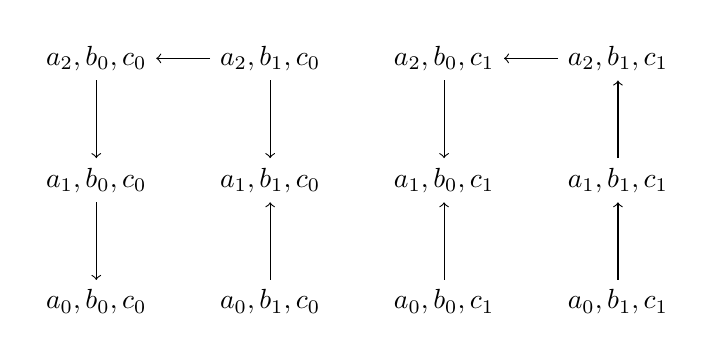
\begin{tikzpicture}
      \matrix [column sep=0.7cm, row sep=1cm]{
        \node (s200) {$\RRBetat{a_2,b_0,c_0}$}; &
        \node (s210) {$\RRBetat{a_2,b_1,c_0}$}; &
        \node (s201) {$\RRBetat{a_2,b_0,c_1}$}; &
        \node (s211) {$\RRBetat{a_2,b_1,c_1}$}; \\
        \node (s100) {$\RRBetat{a_1,b_0,c_0}$}; &
        \node (s110) {$\RRBetat{a_1,b_1,c_0}$}; &
        \node (s101) {$\RRBetat{a_1,b_0,c_1}$}; &
        \node (s111) {$\RRBetat{a_1,b_1,c_1}$}; \\
        \node (s000) {$\RRBetat{a_0,b_0,c_0}$}; &
        \node (s010) {$\RRBetat{a_0,b_1,c_0}$}; &
        \node (s001) {$\RRBetat{a_0,b_0,c_1}$}; &
        \node (s011) {$\RRBetat{a_0,b_1,c_1}$}; \\
      };
      \path[->]
        (s010) edge (s110)
        (s100) edge (s000)
        (s200) edge (s100)
        (s210) edge (s110) edge (s200)
        (s001) edge (s101)
        (s011) edge (s111)
        (s111) edge (s211)
        (s201) edge (s101)
        (s211) edge (s201)
      ;
    \end{tikzpicture}
    \end{center}
    \caption{\figlabel{thomas-dynamique}%
      Représentation de la dynamique du modèle de Thomas donné à la \figref{thomas}.
      Chaque état est représenté par un triplet $\RRBetat{a_i, b_j, c_k}$
      où $i$, $j$ et $k$ représentent respectivement le niveau d'expression de $a$, $b$ et $c$,
      et une transition entre deux états est représentée par une flèche.
    }
  \end{figure}
\end{example}



\subsubsection*{Graphe des interactions minimal}
Il est possible d'inférer le graphe des interactions \emph{minimal} d'un modèle de Thomas,
en ne conservant que les arcs fonctionnels pour la dynamique.
Définissons $f^a(s) = \RRBget{s}{a}$ si $s[a]\in K_{a, \RRBres{a}{s}}$,
et $f^a(s) = \RRBget{s}{a} + \delta^a(s)$ sinon.
Une régulation positive (\resp négative) de $b$ sur $a$ n'est inférée que s'il existe
un état $s$ tel que l'augmentation du niveau de $b$ aurait pour conséquence
une augmentation (\resp diminution) de la valeur de $f^a$ ;
ou, en d'autres termes, s'il existe un état $s$ tel que :
$f^a(s \recouvre b_i) < \text{(\resp $>$) } f^a(s \recouvre b_{i+1})$, 
où $i < l_b$ et $s \recouvre b_i$ est l'état identique à $s$
sauf pour la composante de $b$ qui a été remplacée par $b_i$.
Un tel graphe des interactions peut être utilisé pour inférer des propriétés globales sur
la dynamique \citeaffixed{Richard10,PR11-SASB}{cf. par exemple}.

\subsubsection*{Discussion sur la valeur du plafond}
\label{plafond}
Le plafond $l_a$ d'un composant $a$, qui est le niveau d'expression maximum de $a$,
est généralement choisi comme égal au nombre $\card{\components^+(a)}$
de régulations sortant du nœud $a$ dans le graphe des interactions,
c'est-à-dire le nombre de composants qu'il régule.
En effet, chaque niveau discret dans $\segm{0}{l_a}$ représente un ensemble arbitraire de valeurs
pour une donnée réelle et généralement continue de $a$ (niveau d'activité, concentration, etc.),
et pour laquelle $a$ possède une certaine influence sur plusieurs autres composants qu'il régule.
Ainsi, autoriser des valeurs de $l_a$ plus grandes que $\card{\components^+(a)}$
n'augmente pas l'expressivité du modèle
car plusieurs niveaux d'expression de $a$ auront alors le même rôle au niveau des régulations.
À l'inverse, réduire ce plafond à des valeurs plus petites que $\card{\components^+(a)}$
sous-entendrait que plusieurs seuils de régulations sortant de $a$ sont identiques,
ce qui est biologiquement peu plausible.
Cependant, ces considérations peuvent être ignorées pour des raisons diverses de modélisation,
et nous avons choisi de ne pas contraindre le plafond d'un composant dans ce document
pour des raisons de simplicité.
Ainsi, dans l'exemple de modèle de Thomas de la \figref{thomas},
il serait suffisant d'avoir $l_a = 1$ (et $\arc{a}{-}{1}{b} \in E$)
étant donné que $a$ ne possède qu'une régulation sortante.
La valeur $l_a = 2$ permet cependant de rendre l'exemple plus intéressant
en montrant notamment l'aspect unitaire de la dynamique du modèle de Thomas
(et $\arc{a}{-}{2}{b} \in E$ peut être choisi arbitrairement).

\subsubsection*{Discussion sur les signes}
L'ajout d'arcs non-signés ($\uns$) permet de modéliser des régulations dont la tendance générale
est plus complexe qu'une simple activation ou inhibition.
Il est à noter qu'utiliser $\uns$ comme signe pour étiqueter les régulations en plus
des deux signes habituels $+$ et $-$ n'augmente pas l'expressivité du formalisme.
En effet, les signes n'ont pas d'impact sur la paramétrisation (\defref{thomas-param})
ou sur la dynamique (\defref{thomas-dynamique}).
Ils ont cependant un but informatif, car ils résument les différentes régulations du modèle.
Ils seront d'ailleurs utilisés au \chapref{expressivite}
comme base pour énumérer des paramétrisations incomplètes.
Les arcs non-signés seront de plus exploités pour modéliser un graphe des interactions
avec une connaissance partielle de certaines régulations.
Cependant, comme ils ne sont pas courants dans la littérature,
l'état de l'art de la section suivante portera principalement
sur les modèles de Thomas sans arcs non-signés ($E_\uns = \emptyset$).

%\todo{Hypothèses monotonie / etc.}

\subsubsection*{Discussion sur les intervalles de paramètres}
Tandis que la littérature utilise principalement des paramètres entiers
(c'est-à-dire comportant une unique valeur, par exemple : $K_{a,\omega} = i$)
nous proposons ici d'utiliser des intervalles comme valeurs des paramètres
(par exemple : $K_{a,\omega} = \segm{i}{j}$).
Ces intervalles permettent notamment de faciliter la représentation,
bien qu'il soit intéressant de noter qu'ils augmentent l'expressivité du modèle de Thomas.
En effet, considérons un cas fictif où $K_{a,\omega} = \segm{i}{i+2}$
(c'est-à-dire un intervalle contenant trois valeurs) et $s$ un état tel que
$\RRBres{a}{s} = \omega$.
D'après la \defref{thomas-dynamique}, si $\RRBget{s}{a} \in K_{a,\omega}$, alors $a$
ne peut pas évoluer dans $s$ ; ainsi, $a$ possède trois états locaux stables :
$a_i$, $a_{i+1}$ et $a_{i+2}$.
Ce comportement ne peut pas être retrouvé à l'aide de paramètres entiers,
car il n'est pas possible de distinguer les trois configurations de ressources
correspondant aux trois états locaux.
Au plus deux états stables locaux peuvent être créés à l'aide d'une auto-régulation positive
sur $a$ pour distinguer deux configurations différentes
($\RRBget{s}{a} < t$ et $\RRBget{s}{a} \geq t$)
ce qui n'est cependant pas suffisant pour obtenir trois états stables.



\subsection{Définition des réseaux discrets asynchrones}
\seclabel{rda-def}

Certaines contraintes propres aux modèles de Thomas peuvent être relâchées pour permettre
des comportements supplémentaires.
Ainsi, il est courant de représenter des réseaux de régulation biologique
sous la forme de \emph{réseaux discrets asynchrones}.
Ces réseaux sont aussi fondés sur un graphe des interactions,
mais il utilisent des fonctions d'évolution (\defref{rda-def}) pour plus de permissivité,
en lieu et place de paramètres discrets tels que précédemment
formalisés à la \vdefref{thomas-param}.
Par ailleurs, l'hypothèse d'asynchronisme est conservée car un seul composant peut évoluer
depuis chaque état,
mais leur dynamique n'est pas unitaire dans le cas général
car ce composant peut évoluer d'un nombre arbitraire de niveaux d'expression
(\defref{rda-dynamique}).

\begin{definition}[Réseau discret asynchrone ($\RDA$)]
\deflabel{rda-def}
  Si $\GI = (\components; E)$ est un graphe des interactions,
  un \emph{réseau discret asynchrone} est un couple $\RDA = (\GI; F)$
  avec $F = (f_x)_{x \in \components}$, tels que
  $\forall x \in \components, f_x : \RRBreg{x} \rightarrow \segm{0}{l_x}$.
\end{definition}

\begin{definition}[Dynamique d'un réseau discret asynchrone ($\RRBtransrda{}{}$)]
\deflabel{rda-dynamique}
  Pour tout réseau discret asynchrone $\RDA = (\GI; F)$,
  La dynamique non-unitaire de $\RDA$ est donnée par la relation de transition
  $\RRBtransrda{}{}\ \in \RRBstates \times \RRBstates$ définie par :
  \begin{align*}
    \forall s, s' \in \RRBstates, \RRBtransrda{s}{s'}
      &\Longleftrightarrow \exists a \in \components,
    \RRBget{s}{a} \neq f_a(s) \wedge
      \RRBget{s'}{a} = f_a(s) \\
      &\qquad\quad \wedge \forall b \in \components, b \neq a \Rightarrow \RRBget{s}{b} = \RRBget{s'}{b}
  \end{align*}
\end{definition}

Enfin, nous désignons par \emph{réseau booléen asynchrone}
tout réseau discret asynchrone dont les composants ne possèdent que deux niveaux discrets,
c'est-à-dire tel que : $\forall x \in \components, l_x = 1$.



\subsection{Analyses formelles du modèle de Thomas}
\seclabel{thomas-analyse}

Nous proposons dans cette section un tour d'horizon rapide des différentes méthodes
d'analyse de la dynamique des modèles de Thomas.
Nous nous concentrons principalement sur les méthodes d'analyse statique,
c'est-à-dire permettant d'obtenir des résultats sur la dynamique d'un modèle
sans nécessiter d'en calculer la dynamique de façon complète et explicite.
Ces approches ont l'avantage de jouir d'une faible complexité, même si les résultats formels
qu'elles fournissent sont généralement moins précis ou approximés.
L'analyse du graphe des interactions seul peut ainsi permettre d'obtenir certains
résultats sur sa dynamique,
et la prise en compte de la paramétrisation permet d'affiner cette approche.
Cependant, ces résultats sont insuffisants dans beaucoup de cas,
nécessitant des approches plus exhaustives.
L'analyse complète de la dynamique d'un modèle de Thomas
est généralement invoquée en dernier recours, car elle peut être coûteuse en temps
et en espace mémoire du fait de l'explosion combinatoire inhérente au calcul
de l'espace des états.

\subsubsection*{Analyse du graphe des interactions}
Plusieurs travaux se sont intéressés aux conclusions qui pouvaient être
tirées du seul graphe des interactions.
La recherche d'\emph{états stables}, aussi appelés \emph{points fixes},
présente un intérêt particulier dans l'étude des réseaux de régulation biologique
et a été de fait très étudiée.
Les conjectures de \citefullname{Thomas81}{René}
tracent notamment un lien entre la présence de circuits dans les régulations et celle
d'oscillations ou d'états stables.
Elles se formulent comme suit :
\begin{itemize}
  \item un circuit positif (c.-à-d.~comportant un nombre pair de régulations négatives)
    est une condition nécessaire à la présence de plusieurs points fixes,
  \item un circuit négatif (c.-à-d.~comportant un nombre impair de régulations négatives)
    est une condition nécessaire à la présence d'oscillations dans la dynamique.
\end{itemize}
Ces conjectures ont par la suite été démontrées
dans le cas booléen, c'est-à-dire lorsque $\forall x \in \components, l_x = 1$
\cite{RRT08,Richard06thesis}
ainsi que dans le cas multivalué \cite{RiCo07,Richard10}.

Plusieurs résultats viennent de surcroît enrichir ce résultat concernant
l'existence de points fixes.
Des travaux ont par exemple
permis d'obtenir une valeur maximale du nombre de points fixes possibles
dans un modèle de Thomas tant booléen \cite{aracena2008maximum} que multivalué \cite{Richard09}.
Cette valeur dépend du nombre de composants à supprimer pour éliminer
tout circuit positif dans le modèle.
\citeasnoun{PR10-CRAS} ont quant à eux proposé une valeur minimale du nombre de
\emph{points fixes topologiques} d'un modèle booléen.
Ces points fixes ont la particularité de ne pas dépendre de la paramétrisation,
ce qui permet de généraliser un tel résultat à un ensemble de modèles de Thomas.

\subsubsection*{Analyse de la paramétrisation}
Les conditions données précédemment sont \emph{nécessaires} mais non \emph{suffisantes}
pour observer l'apparition des comportements décrits (oscillations et multistationnarité).
Plusieurs travaux permettent d'analyser la fonctionnalité des circuits,
c'est-à-dire leur capacité à effectivement «~générer~» ces comportements,
et donc de rendre ces conditions susnommées nécessaires.
Partant d'un modèle de Thomas donné,
il est possible de représenter sa paramétrisation
à l'aide de diagrammes de décision binaires ou multivalués \cite{Bryant86,Srinivasan90}
afin d'en déduire
l'ensemble des états stables mais aussi d'analyser la fonctionnalité des circuits
en effectuant des produits de diagrammes de décision \cite{Naldi07}.
Les différentes façons dont les oscillations et la multistationnarité sont «~générées~»
ont aussi été étudiées, ce qui a permis de préciser ces conditions \cite{Comet13}.

% Compression des paramètres : \cite{Naldi07}
%   qui utilisent des BDD : \cite{Bryant86,Srinivasan90}
% Permet certaines analyses efficaces : points fixes et fonctionnalité des circuits

% \subsubsection*{Caractérisation et recherche des points fixes}
% 
% \todo{dispatcher}
% 
% La recherche d'\emph{états stables}, aussi appelés \emph{points fixes},
% présente un intérêt particulier dans l'étude des réseaux de régulation biologique.
% Les conjectures de \citefullname{Thomas81}{René},
% qui ont par la suite été démontrées \cite{RiCo07}
% portent notamment sur ces questions
% en formulant une condition nécessaire à l'existence de plusieurs points fixes.
% Cette condition n'est cependant pas suffisante
% et ne renseigne pas sur le nombre de points fixes.
% %Dans le cadre d'un modèle booléen (tel que $\forall x \in \components, l_x = 1$)
% L'analyse des interactions seules permet de donner une limite supérieure au nombre
% de points fixes \cite{aracena2008maximum,Richard09}
% ainsi que du nombre de points fixes topologiques,
% (c'est-à-dire ne dépendant pas des paramètres) dans le cas booléen
% \cite{PR10-CRAS},
% sans pour autant proposer une énumération exhaustive.
% \citeasnoun{Naldi07} ont proposé une méthode efficace
% basée sur l'utilisation de diagrammes de décision binaires
% pour l'énumération des points fixes.

\subsubsection*{Analyse de la dynamique}
Afin d'obtenir des résultats plus précis sur le comportement d'un modèle,
comme l'activation d'un composant ou la présence d'oscillations sur une partie
donnée du modèle,
ce que les méthodes décrites précédemment ne permettent pas d'obtenir,
il peut devenir nécessaire de faire appel à des techniques
de \textit{model checking} plus poussées
\citeaffixed{Richard06,gallet14adapting}{voir p.~ex.}.
Ces méthodes permettent généralement une analyse exhaustive de la dynamique,
tout en devant faire face à l'explosion combinatoire typique de ce type d'analyse,
qui limite grandement la taille des modèles étudiés.
De telles analyses ont été théorisées par \citeasnoun{bernot04}
et se basent sur l'expression de propriétés exprimées en logiques temporelles
CTL \cite{Clarke82} ou LTL \cite{Pnueli77}.
Elles possèdent l'avantage d'être très complètes
car la dynamique est entièrement explorée et l'expressivité des logiques temporelles permet
d'exprimer beaucoup de propriétés intéressantes,
mais au prix d'une complexité très importante.
Afin de réduire cette complexité,
\citeasnoun{Naldi09} proposent d'effectuer de la réduction de modèles
en éliminant certaine nœuds qui ont un rôle secondaire.
Le modèle obtenu possède une taille inférieure et certaines bonnes propriétés sont conservées,
comme l'ensemble des points fixes et des attracteurs,
au prix d'une dynamique parfois sous-approximée par rapport au modèle d'origine.
